% Fixture: two-column
% Two-column article on US Letter, like a conference paper: a full-width title
% block and abstract, a full-width figure* at the top of page 2, a
% single-column figure inside the left column, section headings inside
% columns, a footnote at the foot of a column and a short reference list.
%
% Every column ends with an explicit \newpage (which ends the current column
% in twocolumn mode), so the column in which each paragraph appears is fixed
% by this source rather than by TeX's page builder.
\documentclass[10pt,twocolumn]{article}
% Shared settings for every Tourmaline fixture. \input this right after
% \documentclass.
%
% Reproducible output: no creation date, no random trailer id, no pdfTeX
% banner, so rebuilding with the same TeX Live gives byte-identical PDFs.
\pdfinfoomitdate=1
\pdftrailerid{}
\pdfsuppressptexinfo=-1
% Map every glyph (including the fi/fl/ffi ligatures) to Unicode so that
% text extraction does not depend on font-specific guesswork.
\input{glyphtounicode}
\pdfgentounicode=1

\usepackage[letterpaper,margin=0.75in,columnsep=0.3in]{geometry}
\usepackage{float}
\usepackage{tikz}

\title{Column-Aware Reading Order for Scholarly Documents}
\author{Bea Placeholder \and Cyril Sample\\ Institute for Illustrative Research}
\date{}

\begin{document}
\twocolumn[
  \begin{@twocolumnfalse}
    \maketitle
    \begin{abstract}
      Readers of scholarly documents expect text to flow down the left column
      and then down the right one, with titles, abstracts and wide figures
      interrupting that flow where they sit on the page. Software that
      extracts text often gets this wrong. We describe a simple model of
      column structure, explain how wide elements are placed within it, and
      report how often a naive top-to-bottom order goes astray on a small
      collection of papers.
    \end{abstract}
    \vspace{1.5em}
  \end{@twocolumnfalse}
]

% ---------------------------------------------------------------- page 1, left
\section{Introduction}

A two-column page is read as two narrow pages placed side by side. The eye
travels down the left column, returns to the top of the right column, and
continues from there. Anything that spans both columns, such as the title
block above, is read at the point where it appears, before the columns that
follow it.

Extraction tools that sort text purely by vertical position interleave the
two columns line by line, producing sentences that jump back and forth
between unrelated paragraphs.\footnote{This failure is common enough that
many readers have learned to distrust copied text from such papers.} The
problem is easy to state but surprisingly easy to get wrong in practice,
because real pages mix columns, wide floats, footnotes and running headers.

% A figure* declared here floats to the top of the next page.
\begin{figure*}[t]
  \centering
  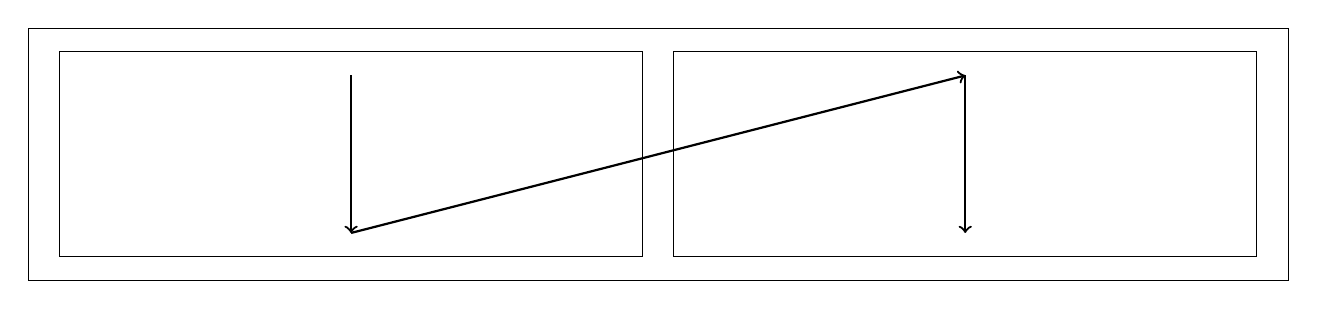
\begin{tikzpicture}[x=10mm,y=10mm]
    \draw (0,0) rectangle (16,3.2);
    \draw (0.4,0.3) rectangle (7.8,2.9);
    \draw (8.2,0.3) rectangle (15.6,2.9);
    \draw[->,thick] (4.1,2.6) -- (4.1,0.6);
    \draw[->,thick] (4.1,0.6) -- (11.9,2.6);
    \draw[->,thick] (11.9,2.6) -- (11.9,0.6);
  \end{tikzpicture}
  \caption{The reading path on a two-column page runs down the left column,
  back up to the top of the right column, and down again. Wide elements
  such as this figure are read where they sit, before the columns below.}
  \label{fig:path}
\end{figure*}

\newpage
% --------------------------------------------------------------- page 1, right
\section{Related Work}

Document layout analysis has a long history in the processing of scanned
office documents, where the input is a raster image and the regions of text
must be found before they can be read. Born-digital documents make the first
step easier, since the characters and their positions are known exactly, but
the grouping of characters into lines, lines into blocks and blocks into a
reading sequence remains the same problem.

\subsection{Layout analysis}

Most methods look for a vertical band of white space that separates the
columns over a large part of the page. Wide elements break that band, and a
robust method has to treat the page as a stack of horizontal regions, each
with its own number of columns, rather than as a single grid.

\newpage
% ---------------------------------------------------------------- page 2, left
\section{Approach}

We first group text items into lines by their baselines, then split each
line where it crosses the gap between the columns. Regions are formed from
runs of consecutive lines that share the same split.

\begin{figure}[H]
  \centering
  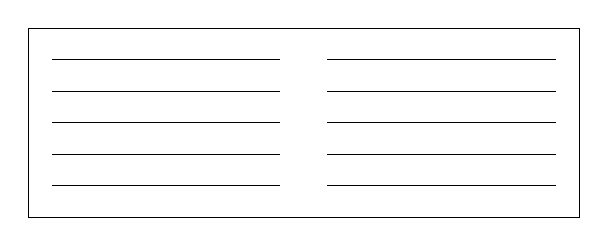
\begin{tikzpicture}[x=10mm,y=10mm]
    \draw (0,0) rectangle (7,2.4);
    \foreach \y in {0.4,0.8,1.2,1.6,2.0} \draw (0.3,\y) -- (3.2,\y);
    \foreach \y in {0.4,0.8,1.2,1.6,2.0} \draw (3.8,\y) -- (6.7,\y);
  \end{tikzpicture}
  \caption{Lines are split at the gap between the columns before regions
  are formed.}
  \label{fig:split}
\end{figure}

Within a region the left column is emitted before the right one. Regions
themselves are emitted from the top of the page to the bottom, so a wide
figure that sits between two bands of columns is read between them.

\newpage
% --------------------------------------------------------------- page 2, right
\subsection{Handling floats}

Figures and tables are treated as blocks rather than as text. A caption is
attached to the float it describes, so that it is read together with the
figure and not as part of the surrounding paragraph.

\subsection{Footnotes and page furniture}

Footnotes are read at the end of the column in which they appear. Running
headers and page numbers are excluded from the reading sequence entirely,
since they repeat on every page and carry no part of the argument.

\newpage
% ---------------------------------------------------------------- page 3, left
\section{Evaluation}

We checked the model against a handful of papers with hand-labelled reading
order. A naive order that sorts lines by their vertical position was wrong on
every two-column page, while the region model was wrong only where a caption
had been set in the margin.

Most remaining errors involved short lines, such as equation numbers and
section headings, whose horizontal position did not clearly place them in
either column.

\newpage
% --------------------------------------------------------------- page 3, right
\section{Conclusion}

Treating a page as a stack of regions with their own column counts handles
the common cases of scholarly layout with very little machinery.

\begin{thebibliography}{9}
\bibitem{doe} J. Doe. Reading order in structured documents. \emph{Journal
  of Placeholder Studies}, 12:1--20, 2001.
\bibitem{roe} R. Roe and S. Poe. White space as a layout cue. In
  \emph{Proceedings of the Sample Workshop}, pages 5--9, 2010.
\bibitem{moe} M. Moe. \emph{A Primer on Page Segmentation}. Example Press,
  2015.
\end{thebibliography}

\end{document}
